\newpage 
\thispagestyle{empty}
\chapter{Implementierung}\label{sec:Implementierung}
Wie bereits im Kapitel \ref{sec:Interpretation_Dipol} erwähnt, wird die Antennenstruktur weder auf eine FR4 Kunstharzplatte noch auf eine Plastikfolie aufgedruckt, da einerseits die Produktionskosten von Kleinserien im Verhältnis zu deren Nutzen unverhältnismässig gross sind und andererseits jeder Fertigungsdurchgang einer gedruckten Antennen mindestens ein bis drei Tage in Anspruch nimmt. Daher werden die zu testenden Antennen aus einer Kupferfolie ausgeschnitten, so können Änderungen im Designs sehr schnell umgesetzt und die Kosten gering gehalten werden.\\

Aufgrund der Resultate der verschiedenen Simulationen einer Dipol Antenne im Kapitel (\ref{sec:Interpretation_Dipol}) wurde entschieden, dass ein Funktionsmuster der Dipol Antenne mit einer Breite von 3 mm und einer Dicke von 26 $\mu m$ sowie einer Länge von 50.25 mm hergestellt wird, um das Abstrahlverhalten auszumessen. Wie die Abbildung \ref{S11_Vergleich_Simulation_Dipolantenn_freiraum_Geraet} zeigt, unterscheidet sich das simulierte Abstrahlverhalten von Dipolen mit einer Breite von 1 mm gegenüber von Dipolen mit einer Breite von 3 mm nur unwesentlich, die Antennenstruktur mit einer Breite von 3 mm ist jedoch wesentlich einfacher zu bearbeiten als die 1 mm breite Antennenstruktur. Das Kupferband mit einer Breite von weniger als 3 mm kann bereits unter geringem Zug reissen, zudem ist eine grössere Fläche von Vorteil, um die Antenne mit Klebstoff an das Kunststoffgehäuse fixieren zu können.  \\
\newpage
Die Antenne wird mittels Skalpell aus dem Kupferklebeband ausgeschnitten. Dabei gilt es zu beachten, dass sich das Kupferband nicht in seine ursprünglicher Form zurückzieht. Abbildung \ref{fig:DipolausKupferband} zeigt die oben beschriebenen Antennenstruktur aus dem Kupferklebeband geschnitten.  Das Zentrum der Antenne dient als Fusspunkt derselben und wird mit einem ca. 1 mm$^{2}$ grosssen Lötzinnpunkt versehen. An diesem speist die Zuleitung in Form eines Koaxialkabels die Antenne.\\
\begin{figure}[!ht]
	\centering
	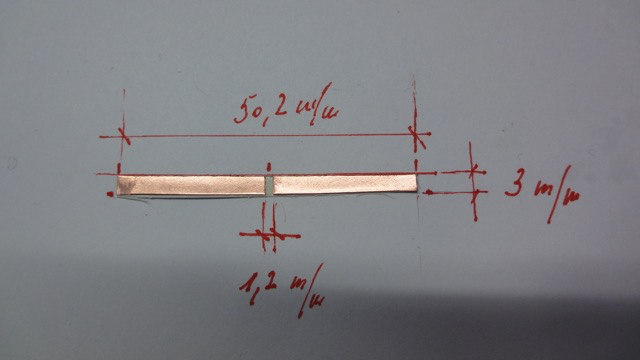
\includegraphics[width=15cm]{content/bilder/Implementierung/Dipol3mm50mm.jpg}%
	\caption{Dipol aus Kupferklebeband ausgeschnitten}
	\label{fig:DipolausKupferband}
\end{figure}

\newpage
In Abbildung \ref{fig:DipolausKupferbandGeraeteinnenseite} ist  die Dipol Antenne mit einem Koaxialkabel als Speiseleitung gezeigt. Das Koaxialkabel dient als längs homogene Leitung. Sie führt die elektromagnetische Welle von der Quelle zur Antenne. Die Leitung wird rechtwinklig von der Antenne weggeführt. Es muss stets darauf geachtet werden, dass der Biegeradius des Koaxialkabels eingehalten wird. Der Aussenleiter des Koaxialkabels muss nicht zusätzlich gegenüber dem darunterliegenden Akkupaket isoliert werden, denn dieser ist bereits in eine Kunststofffolie gehüllt. Jedoch muss darauf geachtet werden, dass der Aussenleiter des Koaxialkabels nicht mir der Elektronikplatine, die sich auf der Rückseite des Displays befindet, kurzschliesst. Daher erfüllt das Papierklebeband mehrere Aufgaben. Es dient als Isolation zwischen der Elektronikplatine und dem Koaxialkabel und zusätzlich als Zugsentlastung der Antenne. Des weitern hilft das Papierklebeband zur Fixierung der Antenne.\\
\begin{figure}[!ht]
	\centering
	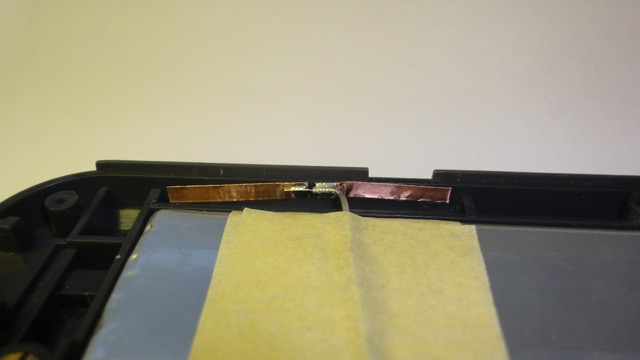
\includegraphics[width=15cm]{content/bilder/Implementierung/DipolIMGeraet.jpg}%
	\caption{Dipol aus Kupferklebeband an der Geräteinnenseite befestigt}
	\label{fig:DipolausKupferbandGeraeteinnenseite}
\end{figure}
\clearpage
\newpage
Die Abbildung \ref{fig:DipolimGeraet} zeigt, wie die Antenne im Fluginstrumet positioniert ist. Aus dieser Abbildung ist sehr gut zu erkennen, dass die Antenne direkt an die Aussenwand des Kunststoffgehäuses  des Fluginstumentes geklebt ist. Das Koaxialkabel führt rechtwinklig von der Antenne weg bis zum SMA-Stecker. Über diesen, wird die Antenne mit der interne Quelle des StarLab verbunden.\\
\begin{figure}[!ht]
	\centering
	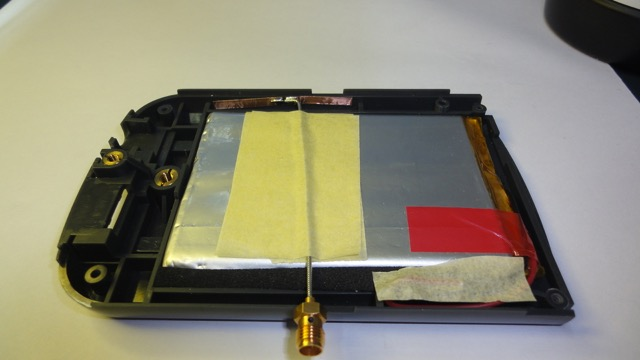
\includegraphics[width=15cm]{content/bilder/Implementierung/DipolKabelGeraet.jpg}%
	\caption{Dipol im Gerät mit Koaxialkabel und SMA-Stecker}
	\label{fig:DipolimGeraet}
\end{figure}






